\documentclass[11pt,spanish]{article}

\usepackage[a6paper, landscape,
	left=1cm, top=1cm, right=1cm, bottom=1.5cm
]{geometry}
%\usepackage[a4paper, margin=3cm]{geometry}
\usepackage{babel}
\usepackage{xltxtra}
\usepackage{grid-system}
\usepackage{multicol} % simpler than grid for lots of cases
\usepackage{hyperref}
\usepackage{xcolor}
\usepackage{graphicx}
\usepackage[export]{adjustbox}
\usepackage{fancyhdr}
\usepackage{listings}

\setmainfont{Comic Sans MS}
%\setmathfont{eulervm}
%\lstset{basicstyle=\footnotesize\ttfamily}
\lstset{basicstyle=\footnotesize\setmainfont{DejaVu Sans Mono}}

\definecolor{verletblue}{HTML}{487AD8}
\definecolor{verletgreen}{HTML}{37DE88}
\definecolor{verletcyan}{HTML}{1AFBFF}

\fancyhead{}
\fancyfoot{}
\fancyfoot[RO]{{\footnotesize \thepage\ de\ \pageref*{lastpage}}}
\renewcommand{\headrule}{}
%\renewcommand{\footrule}{\vbox to 0pt{\hbox to\headwidth{\dotfill}\vss}}
% XXX should find way to use only one right aligned rule...
\renewcommand{\footrule}{{\footnotesize \rule{\textwidth - 5ex}{0pt}\rule{5ex}{1pt}\vss}}
\pagestyle{fancy}

\newcommand{\fr}[1]{%
	\begin{flushright}
		#1
	\end{flushright}
}
%row space
\newcommand{\rowsp}[1][1em]{\vspace{#1}}
\newcommand{\hone}[1]{{\rowsp[0.3em]\noindent\Large #1 \rowsp[0.3em]}}
\newcommand{\htwo}[1]{{\rowsp\noindent\large #1 \rowsp}}
\newcommand{\htworuler}[1]{{%
	\rowsp\noindent\Large #1%
	\\ {\color{verletgreen}\noindent\rule{\textwidth + 2em}{0.5em}}\rowsp%
}}
\newcommand{\hthree}[1]{{\rowsp\noindent\large #1 \rowsp[0.5em]}}
\newcommand{\hfour}[1]{{\rowsp\large #1 \rowsp[0.5em]}}
\newcommand{\for}[1]{{#1 \rowsp}}
\newcommand{\signline}{\rule{\textwidth}{1pt}}
\newcommand{\emptycell}[1][1]{\begin{Cell}{#1}\ \end{Cell}}
%page with single text horizontally and vertically centered
\newcommand{\displaypage}[1]{%
\
\vspace{\stretch{1}}
\begin{center}
\hone{#1}
\end{center}
\vspace{\stretch{1}}
}

%=======================
% specific to presentations
%\newcommand{\myitm}{aoeuaeou}
\newcommand{\myitm}[1]{\begin{itemize}#1\end{itemize}}

\newcommand{\mydesc}[1]{%
	\begin{description}
	\setlength\itemsep{0em}%
	#1
	\end{description}
}
\newcommand{\pros}{\item[pros:]}
\newcommand{\cons}{\item[cons:]}

\setlength{\parindent}{0pt}
\setlength{\parskip}{1ex plus 0.5ex minus 0.2ex}

%=======================

%\renewcommand{\emph}[1]{\emph{#1}}

\title{prometheus}
\author{Abel Camarillo $<$acamari@verlet.org$>$}

\begin{document}

\maketitle
\thispagestyle{empty}

\newpage

\hone{Agenda}

\myitm{
	\item ¿Quién soy?
	\item ¿Qué es prometheus?
	\item Arquitectura
	\item Integración
}

\newpage %===============
\hone{¿Quién soy?}
\begin{Row}
\begin{Cell}{2}
\myitm{
	\item Desarrollador de software desde el 2008 - OpenBSD, perl, C, sh, js
	\item Lead developer en Neuroservices Communications durante 6 años.
	\item Tech Lead en Vordem SA de CV (2018).
	\item Desarrollador freelance desde el 2015 - Verlet.
	\item Maintainer de 21 paquetes en el árbol oficial de OpenBSD -
	\href{http://openports.se/bbmaint.php?maint=acamari@verlet.org}{
	      http://openports.se/bbmaint.php?maint=acamari@verlet.org}
	\item Interés en UNIX, carpintero, $\sim$arte$\sim$ (teatro, poesía, fotografía), cocina, etc...
}
\end{Cell}

%\begin{Cell}{1}
%\ \\ %XXX so image hasn't its bottom to baseline
%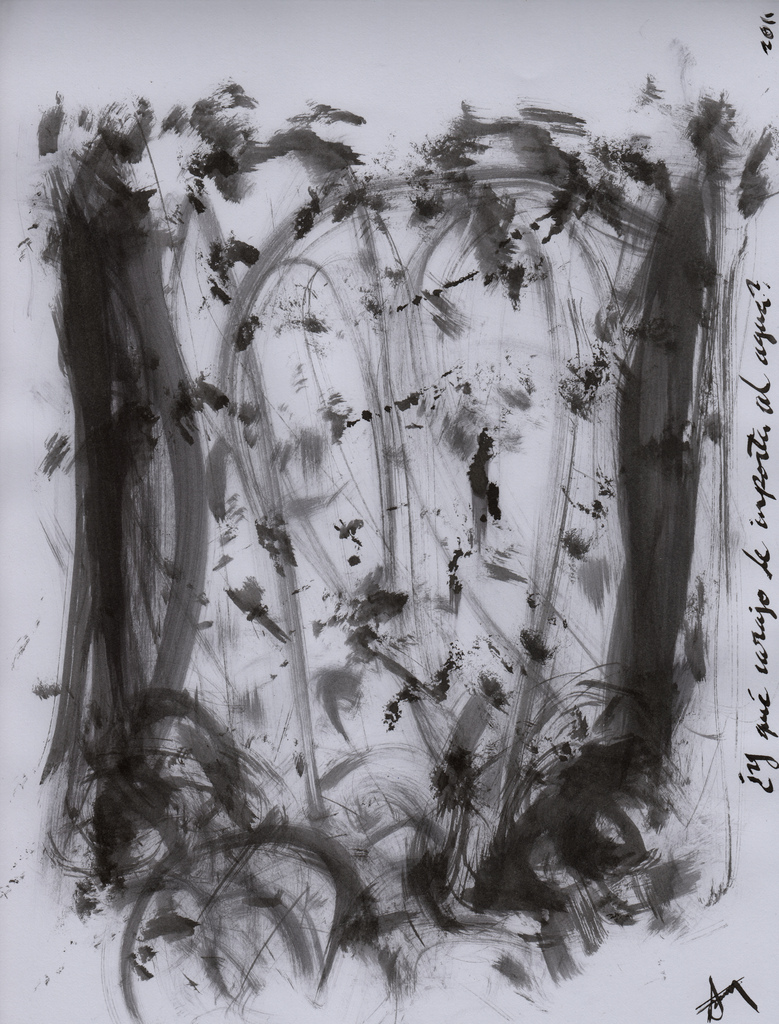
\includegraphics[width=\textwidth]{img/carajo}
%\fr{ {\tiny ¿Y qué carajo\\
%le importa al agua? - 2011} }
%\end{Cell}

\end{Row}


\newpage %===============

\hone{Qué es prometheus}

\myitm{
	\item Producto open source de comunidad
	\item Timeseries database for metrics
	\item indexa llaves, no valores
	\item Prometheus is an open-source systems monitoring and alerting
		toolkit with an active ecosystem. It is the only system directly
		supported by Kubernetes and the de facto standard across the
		cloud native ecosystem. \\
		(verbatim de
		\href{https://prometheus.io/docs/introduction/faq/}{https://prometheus.io/docs/introduction/faq/})
}

%\newpage %===============
%\hone{Qué es loki}
%
%\myitm{
%	\item Producto open source de grafana labs
%	\item Timeseries log aggregator
%	\item inspirado en prometheus (casi idéntico formato de métricas)
%	\item indexa llaves, no valores
%}
%
%Loki is a horizontally scalable, highly available, multi-tenant log aggregation
%system inspired by Prometheus. It is designed to be very cost effective and easy
%to operate. It does not index the contents of the logs, but rather a set of
%labels for each log stream.
%
%The Loki project was started at Grafana Labs in 2018, and announced at KubeCon
%Seattle. Loki is released under the AGPLv3 license.
%
%(de \href{https://grafana.com/oss/loki/}{https://grafana.com/oss/loki/})

\newpage %===============
\displaypage{Arquitectura}

\newpage %===============
\begin{center}
	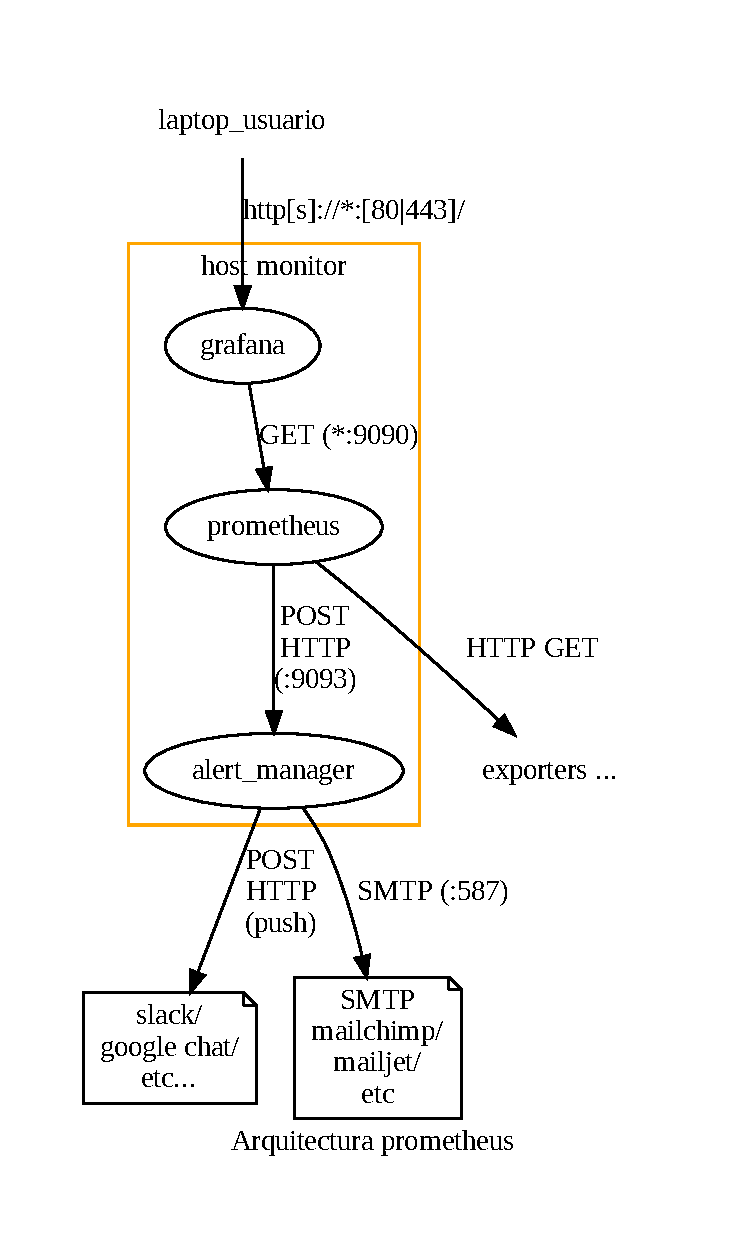
\includegraphics[keepaspectratio=true,width=\textwidth,height=\textheight]{img/prometheus_loki/arq-prometheus}
\end{center}

\newpage %===============
\begin{center}
	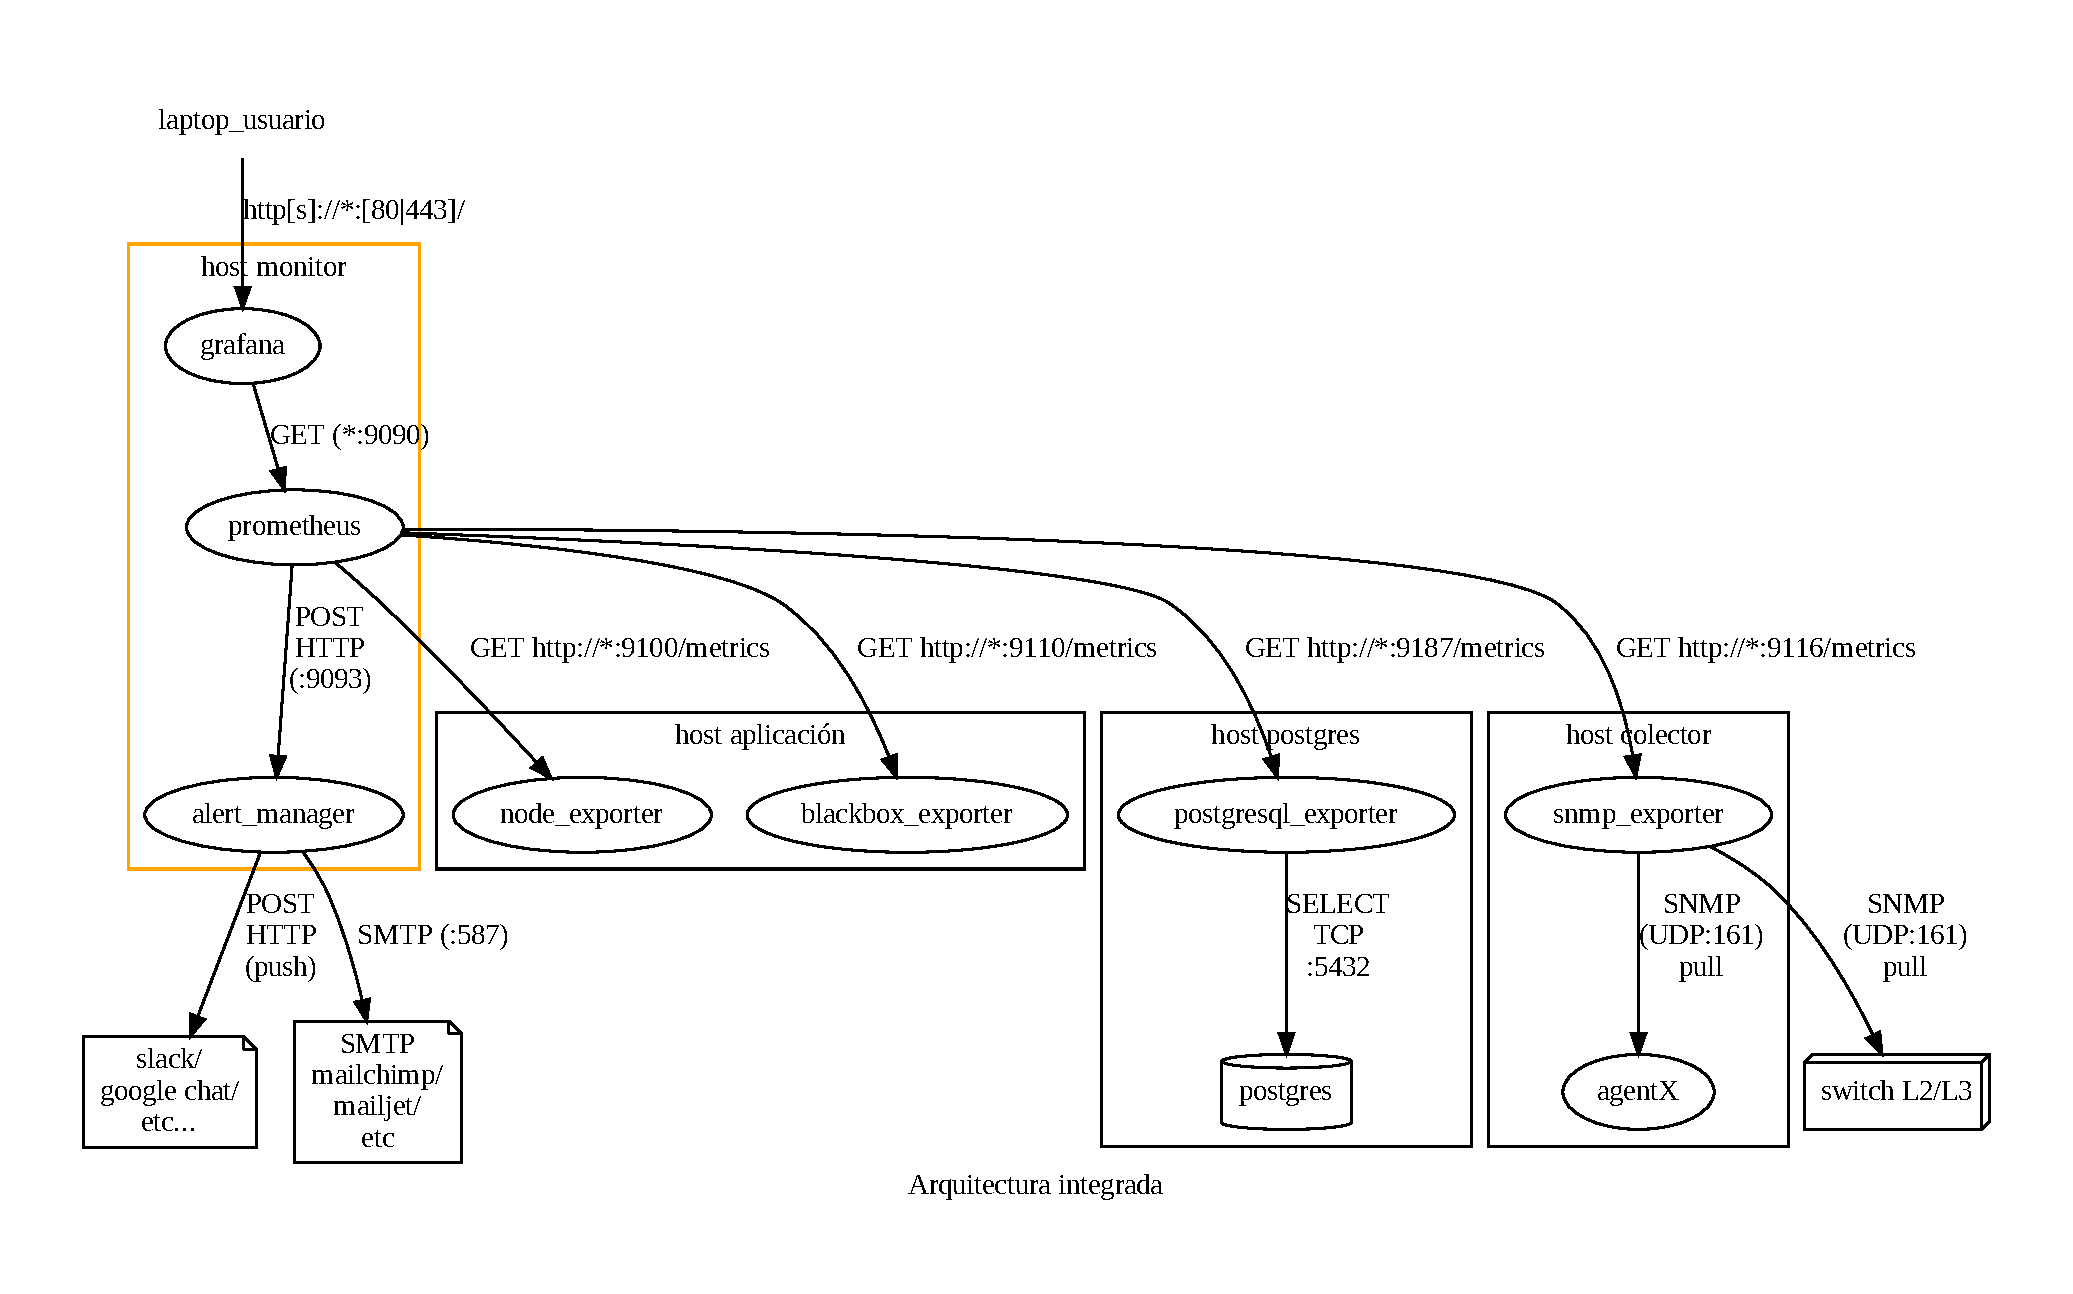
\includegraphics[keepaspectratio=true,width=\textwidth,height=\textheight]{img/prometheus_loki/arq}
\end{center}

\newpage %===============
\hone{Formato de métricas}

V4. Definido en github de prometheus (\textbackslash{} agregados para legibilidad):

\href{https://github.com/prometheus/docs/blob/master/content/docs/instrumenting/exposition_formats.md}{\tiny https://github.com/prometheus/docs/blob/master/content/docs/instrumenting/exposition\_formats.md}

Ejemplo:
\begin{lstlisting}
$ curl http://*:9100/metrics;
...
# HELP node_forks_total Total number of forks.
# TYPE node_forks_total counter
node_forks_total 1.8757377e+07
# HELP node_load1 1m load average.
# TYPE node_load1 gauge
node_load1 1
# HELP node_load15 15m load average.
# TYPE node_load15 gauge
node_load15 1.37
# HELP node_load5 5m load average.
# TYPE node_load5 gauge
node_load5 1.15
# HELP node_uname_info Labeled system information as provided by   \
	the uname
system call.
# TYPE node_uname_info gauge
node_uname_info{domainname="(none)",machine="x86_64",nodename="db4"\
    ,release="4.15.12-x86_64-linode105",sysname="Linux",\
    version="#1 SMP Thu Mar 22 02:13:40 UTC 2018"} 1
# HELP process_cpu_seconds_total Total user and system CPU time \
    spent in seconds.
# TYPE process_cpu_seconds_total counter
process_cpu_seconds_total 2111.27
# HELP node_cpu_seconds_total Seconds the cpus spent in each mode.
# TYPE node_cpu_seconds_total counter
node_cpu_seconds_total{cpu="0",mode="idle"} 2.980243359e+07
node_cpu_seconds_total{cpu="0",mode="iowait"} 8497.06
node_cpu_seconds_total{cpu="0",mode="irq"} 0
node_cpu_seconds_total{cpu="0",mode="nice"} 20709.44
\end{lstlisting}

\newpage %===============
\hone{Formato de métricas}

\myitm{
\item Una métrica puede tener varios valores si hay etiquetas
\item Las etiquetas pueden tener longitud arbitraria
\item Etiquetas pueden variar entre ejecuciones: fs nuevos, tarjetas
	de red o IPs entran y salen, etc
}

\newpage %===============
\hone{Administración}

\myitm{
	\item Configuración vía YAML
	\item Se puede configurar rotación de datos por omisión: \\
		\lstinline{/usr/bin/prometheus --storage.tsdb.retention=180d}
	\item Respaldos vía copia directa del directorio completo de data de
		prometheus \lstinline{/var/lib/prometheus}. Puede ser en vivo.
	\item Todo o nada, no hay respaldos segmentados por host o intervalo de
		tiempo.
	\item No hay escalabilidad multihost integrada
}

\newpage %===============
\hone{Integración}

\myitm{
\item Logueo tradicional: syslog, newsyslog, logrotate, etc
\item Manejo de señales: SIGHUP, SIGINT, etc
\item Manejo atómico de archivos:
	\myitm{
	\item No queremos escribir archivo metrics a medias, porque
		en el resto del stack no se podría distinguir la falta
		de métrica vs archivo a medias
	\item Usar archivo temporal /var/www/pronodebsd/.metrics
	\item \lstinline|rename("./.metrics", "./metrics")|
	}
}

\newpage %===============
\displaypage{¿Preguntas?}

\label{lastpage}
\end{document}
